\documentclass[../main.tex]{subfiles}

\begin{document}

In general, one wishes to achieve a high amount of gain and a small amount of loss for critical phenomena like lasers. However, high loss is not always a undesirable feature. For example, the selection of certain laser wavelengths can be achived with the introdcution of artificial losses for the undesired remaining wavelengths. Investigating this will be the aim of the following section.

\subsubsection{Birefringent tuner}
    \paragraph{Methodology}
        One possible realisation for these losses is using a birefringent quartz crystal ($n_Q \approx\num{1.55}$ for the main laser line of \SI{632.1}{nm}). The setup used in the experiment is shown in figure \ref{fig:5-Aufbau}.

        \begin{figure}[H]
            \centering 
            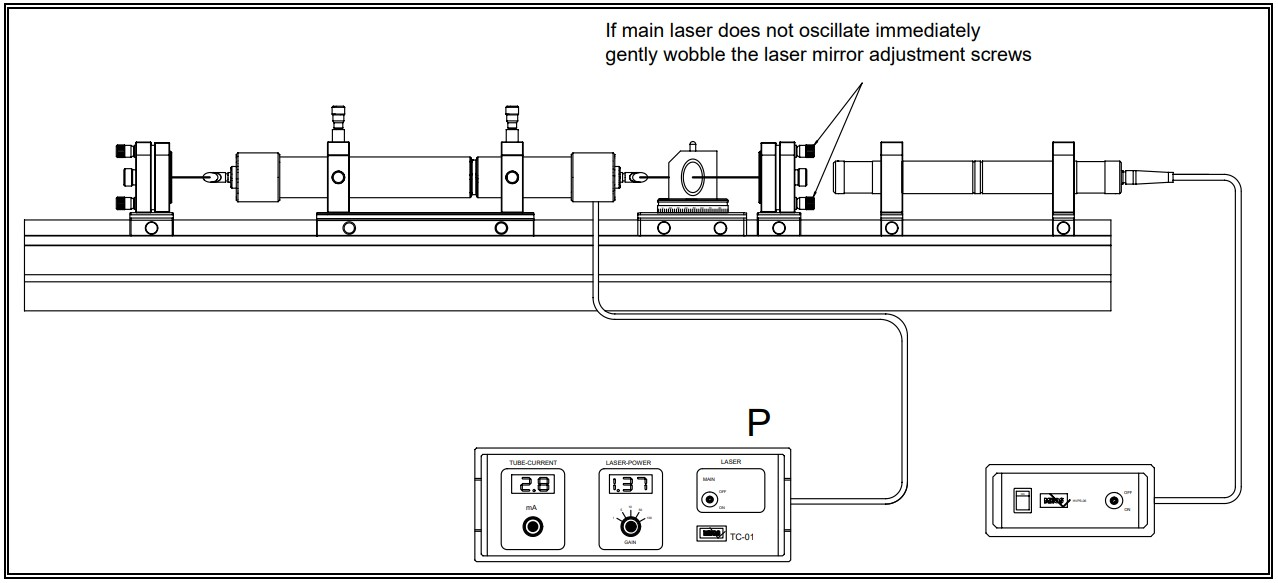
\includegraphics[width = 11cm]{Bilddateien/5/5-Aufbau.jpg}
            \caption{ Experimental setup for the selection of certain laser wavelengths. The components displayed are from left to right: left laser mirror holder (A), main laser tube (B), birefringent tuner (C), right laser mirror holder (D), pilot laser (E). For the measurment of the laser spectrum a spectrometer can be placed left to the left laser mirror holder (A).}
            \label{fig:5-Aufbau}
        \end{figure}

        \noindent The birefringent crystal will be rotated such that the laser light hits the cristal surface at the brewster angle (for \SI{632.1}{nm}) such that no loss is created through reflection. The optical axis should start out vertical to the optical table the laser is built upon. The optical axis is then rotated torwards a horizontal position in steps. For each steps the ordinary and extraordinary ray gather a phase difference when traversing the crystal. Only these wavelengths for which that phase difference is a multiple of $\pi$ do not experience deconstructive interference and are thus selected.

    \paragraph{Data analysis}
        Figure \ref{fig:5-Spektrendoppelbrechung} shows the overlay of two spectra of the laser which were observed to have a peak. 

        \begin{figure}[H]
            \centering 
            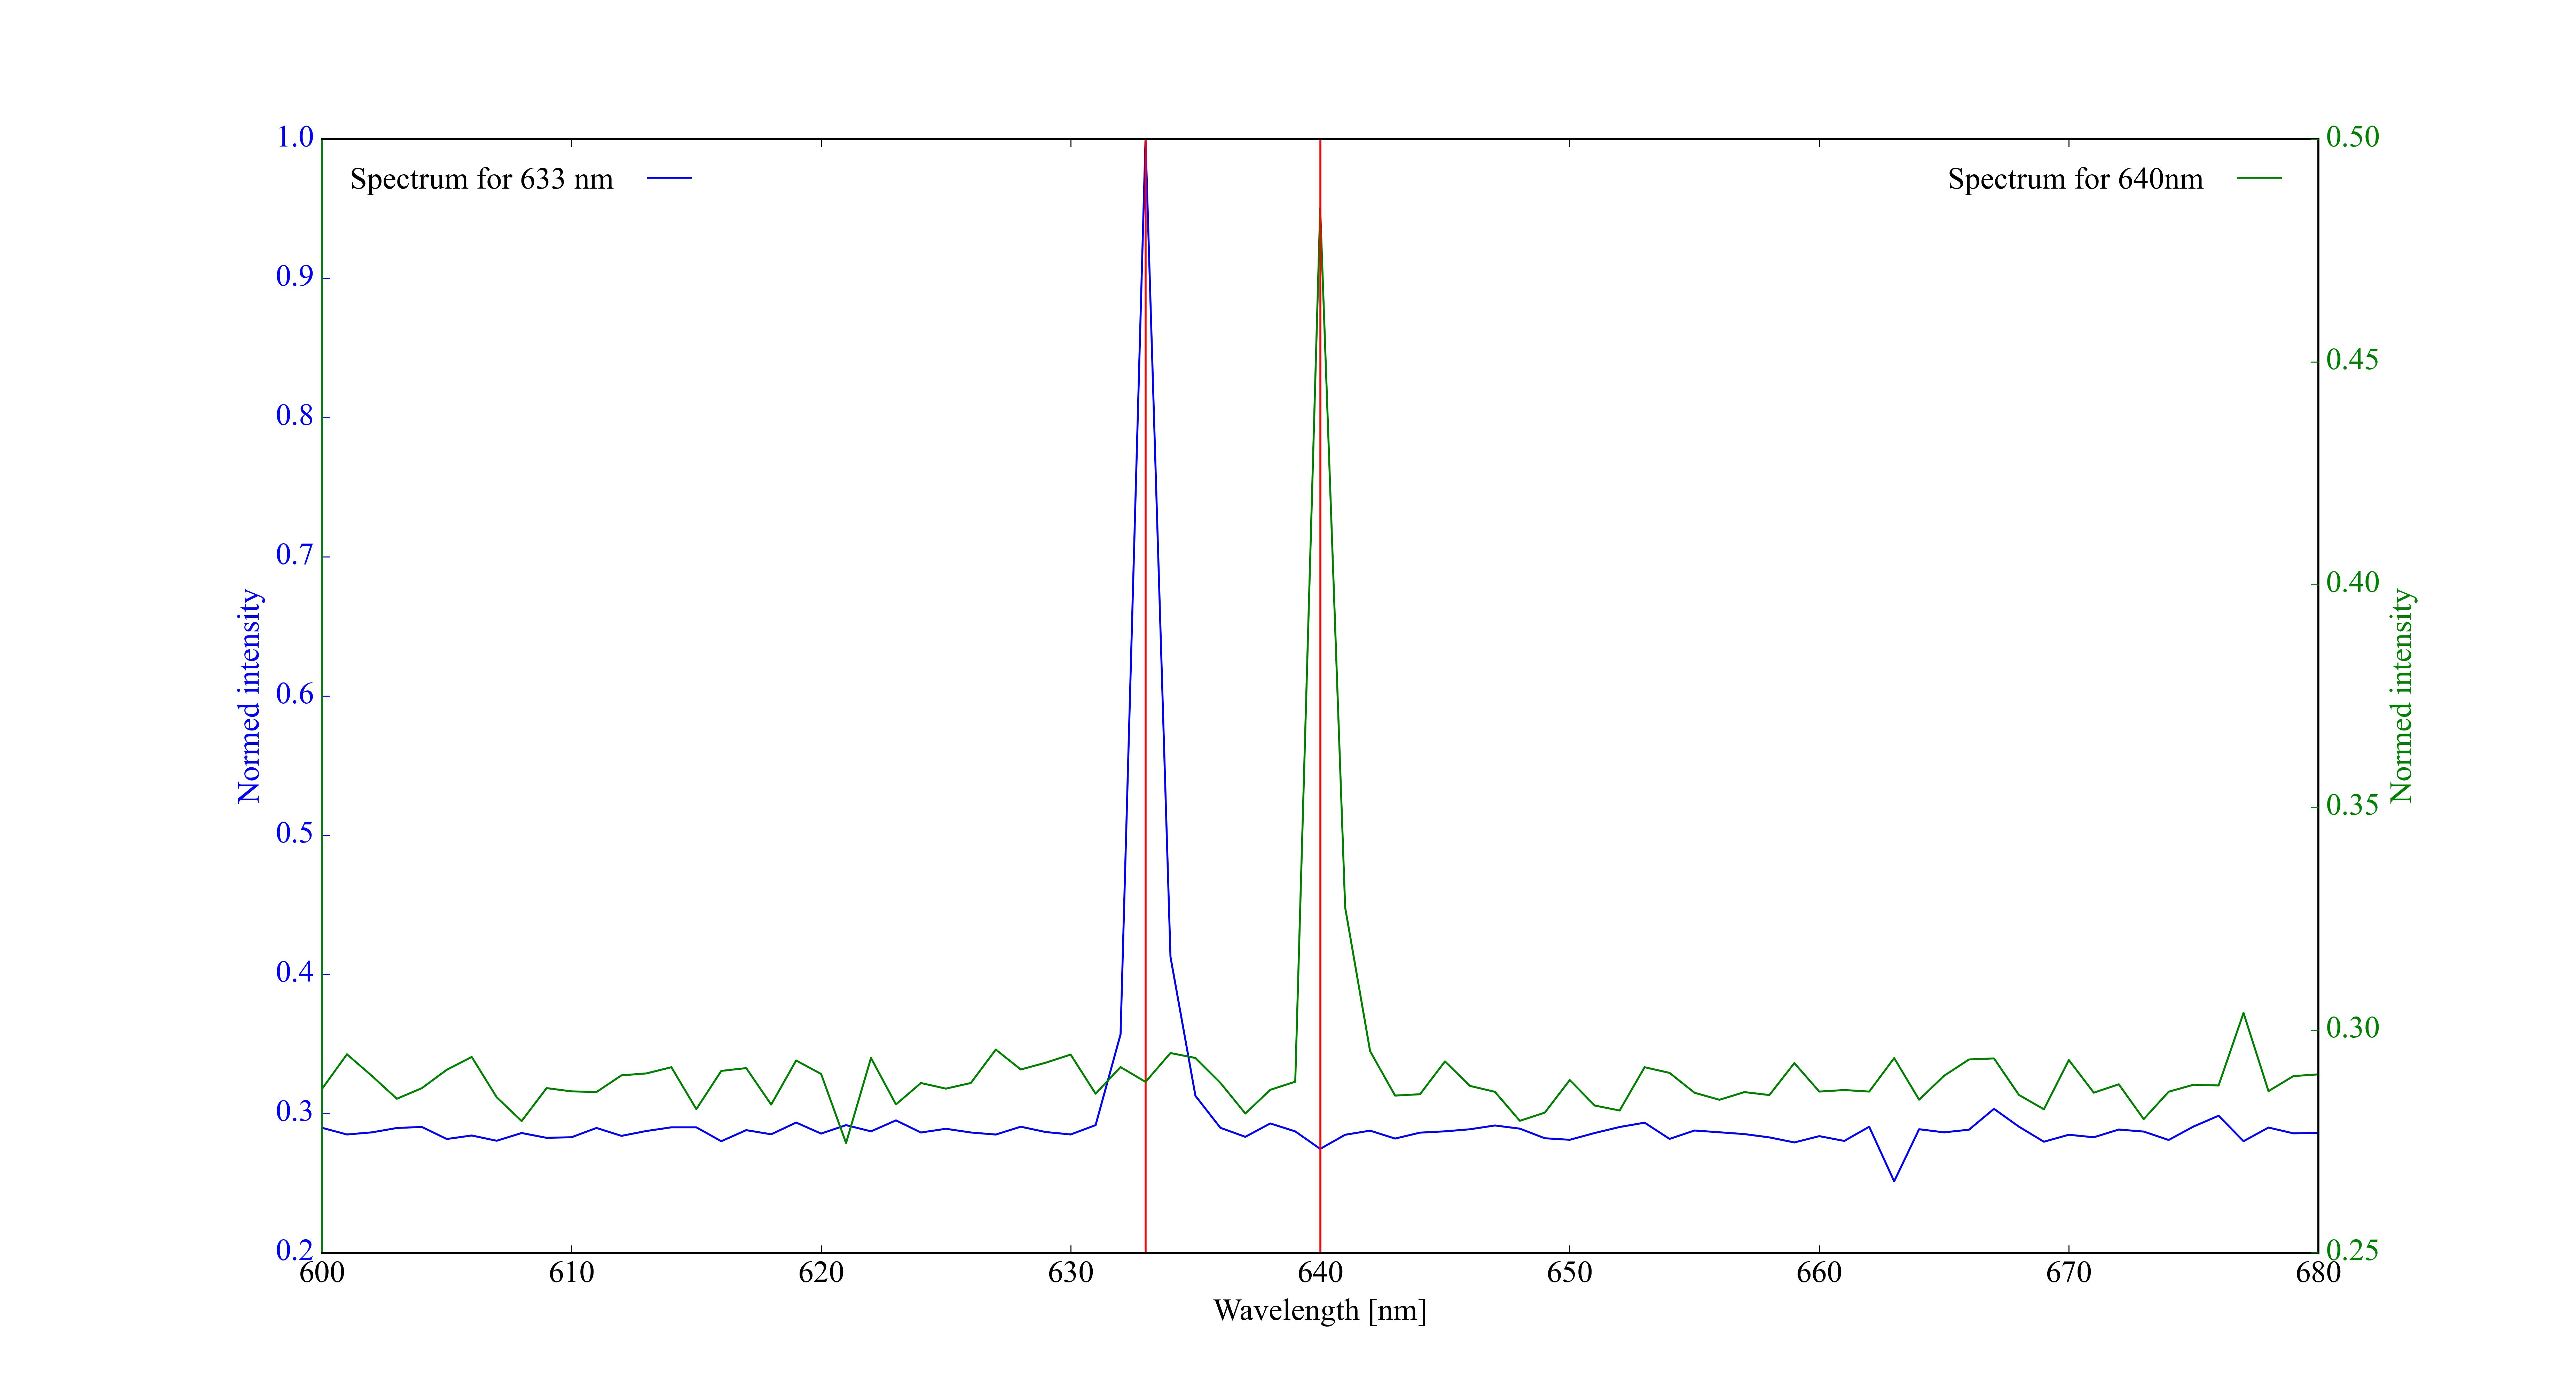
\includegraphics[width = 15cm]{Bilddateien/5/5-Spektrendoppelbrechung.jpg}
            \caption{Filtered spectra of the HeNe-laser (using a birefringent crystal). For two different configurations of the optical axis of the birefringent crystal, a shift in the single appearing spectral peak is seen.}
            \label{fig:5-Spektrendoppelbrechung}
        \end{figure}

        \noindent The observed wavelengths and corresponding probable transitions of Neon gas particle are listed in table \ref{tab:6-Birefringent-peaks}.

        \begin{table}[H]
            \centering 
            \begin{tabular}{c | c c}
                \textbf{wavelength} & \textbf{times observed} & \textbf{correlated transtion}\\\hline\hline
                \SI{633.0(10)}{\nm} & 6 & $3S^2\to 2p^4$\\
                \SI{640.0(10)}{\nm} & 2 & $3S^2\to 2p^2$
            \end{tabular}
            \caption{Observed spectral peaks in the lasing spectrum filtered with a birefringent crystal. The wavelengths listed are mean values of all observed occurences. For the uncertainty the distance between neighbouring Wavelength values in the discretised spectrum.}
            \label{tab:6-Birefringent-peaks}
        \end{table}


\subsubsection{Littrow prism tuner}
    \paragraph{Methodology}
        Another method of introducing loss is to take the basic laser setup (see figure \textbf{ADD REFERENCE!!!}) and replace the mirror in the left mirror holder (A) with a littrow prism. Its functionality is explained in figure \ref{fig:5-FunktionsweiseLitrrowprisma}.

        \begin{figure}[H]
            \centering 
            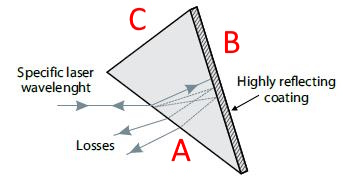
\includegraphics[width = 7cm]{Bilddateien/5/5-FunktionsweiseLitrrowprisma.jpg}
            \caption{Functionality of a littrow prism. Light enters the prism through side A, preferably near the brewster angle to avoid unwanted reflexion. The light is then refracted at side A depending on the wavelength and reflected at the coated side B of the prism. Only for one wavelength reflection occurs at a vertical angle, for all other wavelengths the light rays take a path that leads out of the resonator.}
            \label{fig:5-FunktionsweiseLitrrowprisma}
        \end{figure}

    \paragraph{Data analysis}
        We suceeded in achieving lasing while using a littrow prism and in recording the main laser line. The resulting spectrum is shown in figure . The seperating of other wavelengths did, however, not suceed. It may be that the main laser line had a gain to high in the used laser configuration for other laser transitions to emerge.

        \begin{figure}[H]
            \centering 
            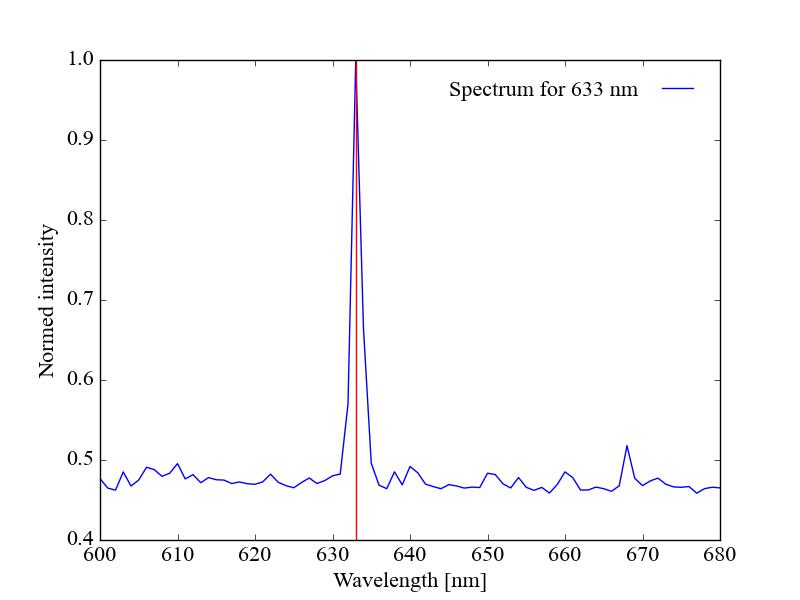
\includegraphics[width = 15cm]{Bilddateien/5/5-Spektrenlittrowprisma.jpg}
            \caption{Filtered spectrum of the HeNe-laser (using a littrow prism). A peak is apparent at \SI{633.0(10)}{\nm}, which is within range of error for the main laser line.}
            \label{fig:5-Spektrenlittrowprisma}
        \end{figure}

\subsubsection{spectra of the laser light}
    \paragraph{Methodology}
    Lastly, a more indirect approach to wavelength 'selection' is taken, which does not focus on actually seperating a single wavelength, but instead on taking the laser spectrum under the microscope. For this, the birefringent crystal (C) is removed from the setup shown in figure \ref{fig:5-Aufbau}. The spectrometer is then placed right next to the main laser tube (B) and a spectrum is taking for two cases: once for when lasing is occuring, and once for when the lasing process is being blocked. The difference between both spectra gives insight into the induced emissions in the Neon gas essential to the function of a laser.

    \paragraph{Data analysis}

    Firstly, the figure shows the laser/ pure fluorescence spectrum for both the case of lasing and no lasing. It is important to note that the spectrum corresponds to that of the light scattered due to \textit{incoherent} emissions in the Neon-Helium gas mixture.

    \begin{figure}[H]
        \centering 
        \includegraphics[width = 11cm]{Bilddateien/5/5-NeonSpektren.jpg}
        \caption{Incoherent scattering spectrum for HeNe-gas. Three main peaks, marked with a red line each, were observed in total.}
        \label{fig:5-NeonSpektren}
    \end{figure}

    \noindent The three larget peaks in figure \ref{fig:5-NeonSpektren} are listed in table \ref{tab:5-NeonSpektren}.

     \begin{table}[H]
        \centering 
        \begin{tabular}{c | c c | c}
            \textbf{wavelength} & \textbf{theoretical laser line} & \textbf{correlated transition} & \textbf{compatible}\\\hline\hline
            \SI{668.0(10)}{\nm} & - & - & -\\\hline
            \SI{588.0(10)}{\nm} & \SI{593.0}{\nm} & $3S^2 \to 2P^8$ & \textcolor{red}{No}\\\hline
            \SI{638.0(10)}{\nm} & \SI{640.1}{\nm} & $3S^2 \to 2P^2$ & \textcolor{red}{No} 
        \end{tabular}
        \caption{Observed main peaks in spetrum \ref{fig:5-NeonSpektren} in order of ascending intensity. For each wavelength, the closest theoretical laser line is matched if one exists within $\pm\SI{5}{\nm}$ of the experimental value.}
        \label{tab:5-NeonSpektren}
     \end{table}

     \noindent The laser line \SI{640.1}{\nm} thus has the highest spontaneous emission rate. One peak at \SI{668.0(10)}{\nm} does not match to any laser line and is possible due to transitions in helium molecules. Interestingly, the main laser line at \SI{632.1}{\nm} does not appear at all as a peak, much less as a one of the three largest peaks.\\

     \noindent For a identification of all laser lines, the difference of the spectrum for no lasing and lasing is shown in figure \ref{fig:5-NeonspektrumDifferenz}.

     \begin{figure}[H]
        \centering 
        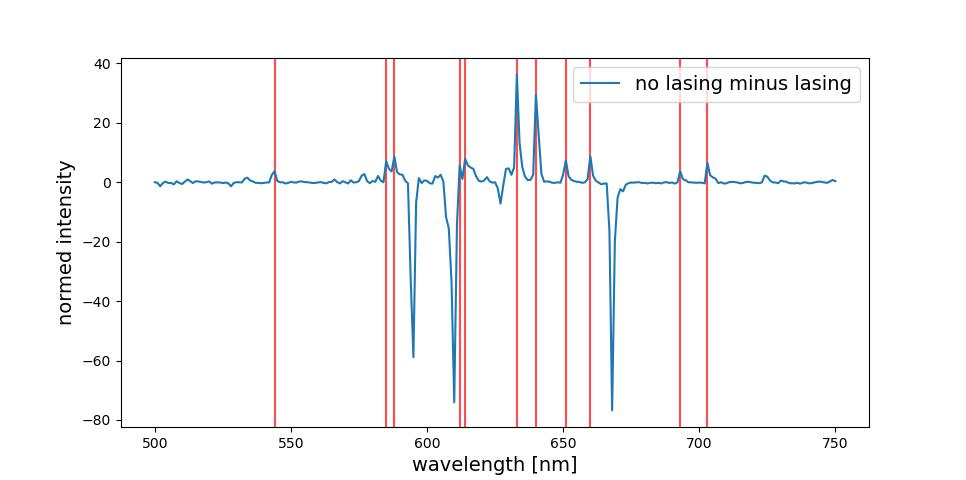
\includegraphics[width = 11cm]{Bilddateien/5/5-NeonspektrumDifferenz.jpg}
        \caption{Fluorescence spectrum for HeNe-gas when lasing is active. Peaks are marked with red lines, valley with green lines.}
        \label{fig:5-NeonspektrumDifferenz}
    \end{figure}

    \noindent As expected, this spectrum has mostly positive values, meaning the fluorescence of the HeNe-gas is less intense during lasing. This can be explained by the fact that more \textit{coherent} emissions are happening and competing with spontaneous emission. For coherent emission in direction of the light oscillating in the resonator, the photons have no possibility to randomly scatter into the direction of the spectrometer. 
    
    However, there are three valleys with negative intensity, meaning an increase for incoherent scattering. This is because due to induced emission a higher photon population is present when lasing, which means more absorption is occuring. These transitions that cannot be meaningfully affected by induced emission thus occur more often through spontaneous, incoherent emission during lasing.\\
    
   \noindent For more detail, all observed spectral lines are listed in table

    \begin{table}[H]
        \centering 
        \begin{tabular}{c | c c | c}
            \textbf{wavelength} & \textbf{theoretical laser line} & \textbf{correlated transition} & \textbf{compatible}\\\hline\hline
            \SI{693.0(10)}{\nm} & - & - & - \\\hline
            \SI{544.0(10)}{\nm} & \SI{543.3}{\nm} & $3S^2 \to 2P^{10}$ & \textcolor{ForestGreen}{Yes}\\\hline
            \SI{612.0(10)}{\nm} & \SI{611.8}{\nm} & $3S^2 \to 2P^6$ & \textcolor{ForestGreen}{Yes}\\\hline
            \SI{703.0(10)}{\nm} & - & - & - \\\hline
            \SI{585.0(10)}{\nm} & - & - & - \\\hline

            \SI{651.0(10)}{\nm} & - & - & - \\\hline
            \SI{614.0(10)}{\nm} & - & - & - \\\hline
            \SI{588.0(10)}{\nm} & \SI{593.9}{\nm} & $3S^2 \to 2P^8$ & \textcolor{red}{No} \\\hline
            \SI{660.0(10)}{\nm} & - & - & - \\\hline
            \SI{640.0(10)}{\nm} & \SI{640.1}{\nm} & $3S^2 \to 2P^2$ & \textcolor{ForestGreen}{Yes}\\\hline

            \SI{633.0(10)}{\nm} & \SI{632.8}{\nm} & $3S^2 \to 2P^4$ & \textcolor{ForestGreen}{Yes}\\\hdashline
            \SI{668.0(10)}{\nm} & - & - & -\\\hline
            \SI{610.0(10)}{\nm} & - & - & -\\\hline
            \SI{595.0(10)}{\nm} & - & - & -\\\hline
            \SI{627.0(10)}{\nm} & - & - & -
        \end{tabular}
        \caption{Observed spectral lines in spetrum \ref{fig:5-NeonSpektren} in order of ascending intensity. The dashed line acts as a separator between peaks and valleys. For each wavelength, the closest theoretical laser line is matched if one exists within $\pm\SI{5}{\nm}$ of the experimental value.}
        \label{tab:5-NeonSpektren}
     \end{table}

     \noindent In total, five of the observed peaks can be matched to Neon transitions. All valleys cannot be matched to laser lines, which is sensible since if they actually were laser lines, they would be affected by induced emission and could not have a higher spontaneous emission rate during lasing.\\
     
     \noindent The order of five matching peaks intensity in which they were listed in matches that of the einstein coefficient for the corresponding state transitions. The only exception is the line \SI{544.0(10)}{\nm}, which is the smallest peak in the sprectrum but whoose einstein coefficient is higher than those for \SI{612.0(10)}{\nm} and \SI{588.0(10)}{\nm}.

\end{document}